%!TEX root = ../2018-10.tex

\chapter{Design Details for Evolution Scenarios}
\label{c:design}
In this chapter we provide the detailed design documentation for each of the evolution scenarios introduced in the previous section. 
Sec.~\ref{App} sketches the design decision for the Mobile App that provides a second sales channel next to the existing Pick-up Shop. Sec.~\ref{Docker} describes the adaptive changes of using a Docker environment to simplify the update process. They are both based on, or at least use the Hybrid Cloud-based Variant of \CoCoME~\cite{HeinrichRostamiReussner2016_1000052688}. In contrast, Sec.~\ref{MS} provides a detailed design documentation of a new architectural version of \CoCoME. This perfective evolution scenario is realized based on the \deleted{M}\added{m}icroservice idea.

\section{Adding a Mobile App Client} 
\label{App}
Developing the Mobile App Client as an extension of \CoCoME requires additional use cases. They are described in Sec.~\ref{UseCasesMobileApp}. Further, Sec.~\ref{DesignMobileApp} describes extensions on design level. The content of this chapter mainly originates from~\cite{schnabel}.

\subsection{Use Cases of the Mobile App}
\label{UseCasesMobileApp}
\begin{figure}[t]
	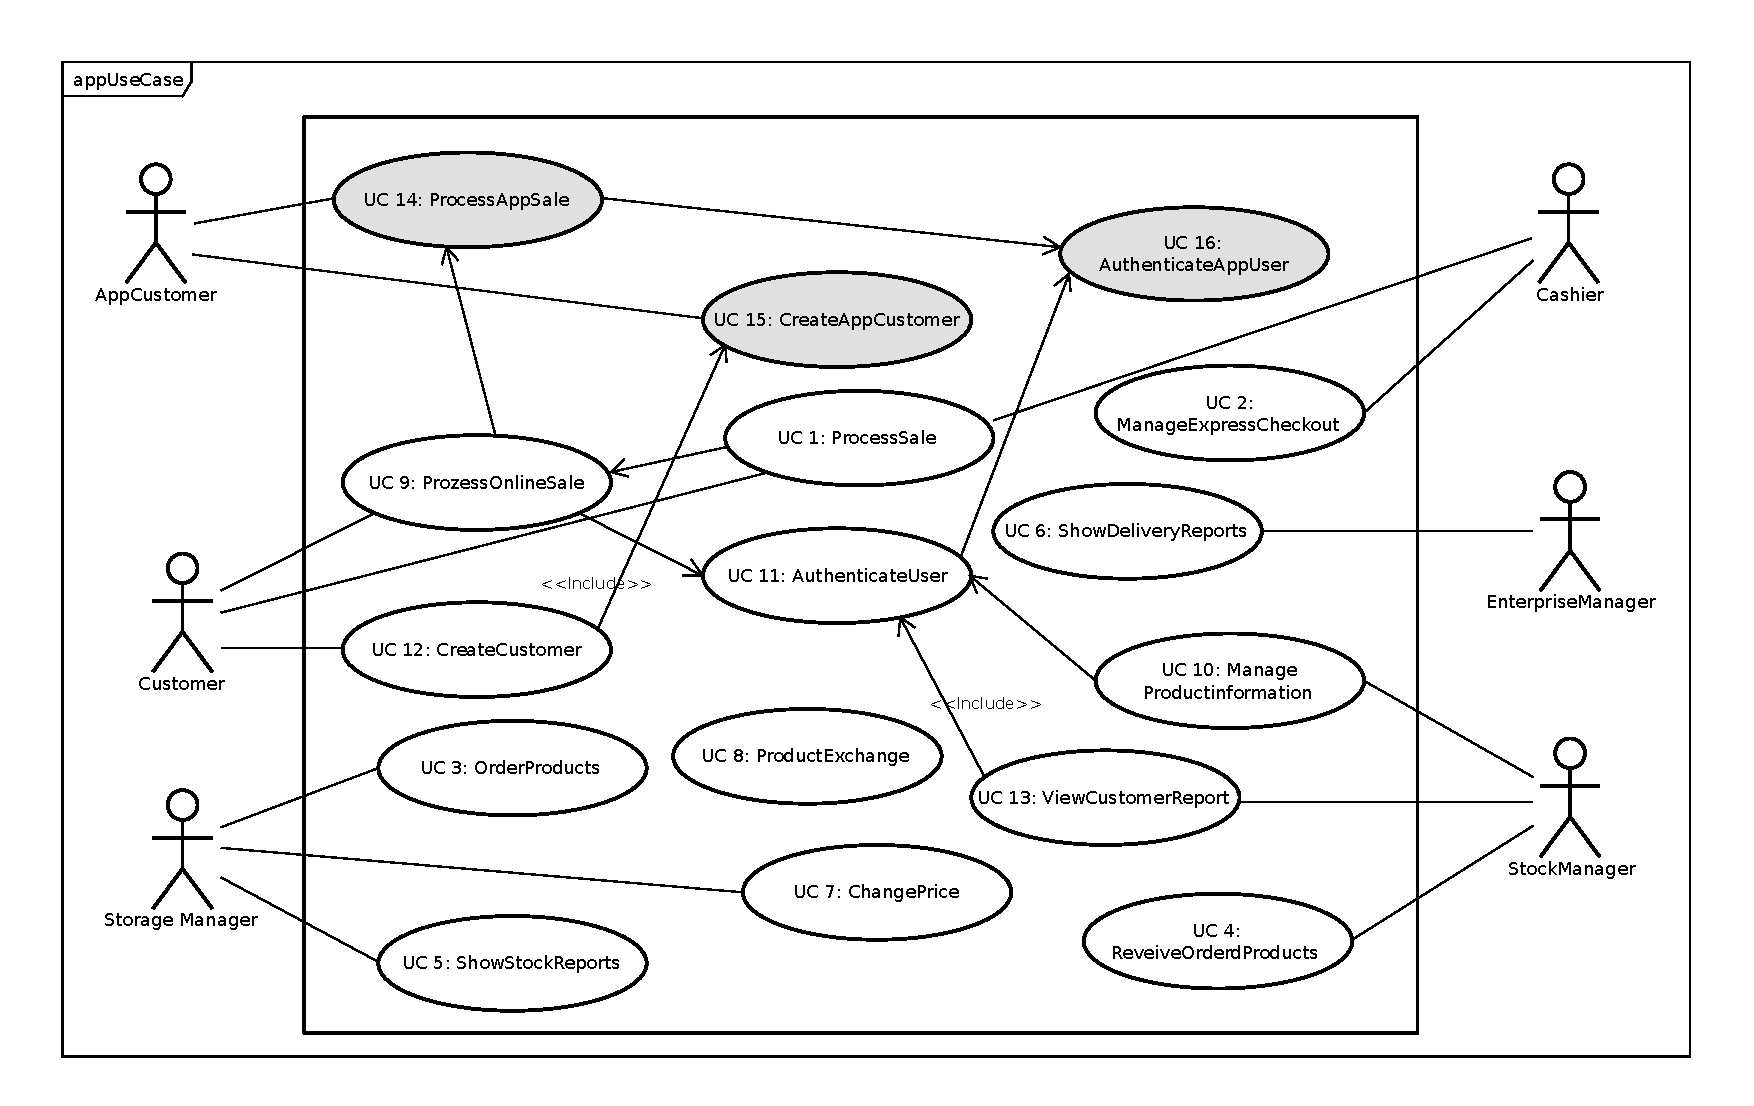
\includegraphics[width=\textwidth]{img/appUseCase.pdf}
	\caption{Use Case Diagram \CoCoME Mobile App}
\end{figure}

\textbf{UC 14 - ProcessAppSale}
\begin{description}[font=\normalfont\itshape]

\item[Brief Description] A Customer selects the product items s/he wants to buy and the payment by credit card is performed.

\item[Involved Actors] AppCustomer, Bank

\item[Precondition] The App is ready to process a new sale and the Customer already has an account registered in the System.

\item[Trigger] The Customer opens the app and wants to buy product items.

\item[Postcondition] The Customer has paid and the sale is registered in the inventory.

\item[Standard Process]

\begin{enumerate}[leftmargin=.5cm]
\item[]
	\item The AppCustomer searches products provided by the App.
	\item The AppCustomer can see details for each product on a separate site.
	\item The AppCustomer adds the product items s/he wants to purchase to the Shopping Cart. Step 1-3 is repeated until all items are added to the cart.
	\item The AppCustomer gets an overview of the items in the cart, their price and the running total.
	\item The AppCustomer proceed to the Checkout 
	\item The AppCustomer selects the Store where s/he wants to pick up his/her	purchased product items. 
	\item The AppCustomer is presented with a login form and is required to complete the "Authenticate user" use case.
	\item In order to initiate card payment, the customer selects a credit card used for the purchase.
	\item The AppCustomer enters his/her PIN in the designated field presented by the System.
	\item The System presents the Customer with an overview of the purchase, the AppCustomer confirms the purchase and waits for validation. Step 9 is repeated until the validation is successful or the Customer decides to cancel the purchase.
	\item Completed sales are logged by the System and sale information are sent to	the Inventory in order to update the stock.
	\item A success message is presented to the AppCustomer and the product items
	are being prepared to be picked up by the customer.
	\item The AppCustomer closes the app.
\end{enumerate}

\item[Alternative or Exceptional Processes]
\begin{itemize}[leftmargin=.3cm]
\item[]
\item \textit{In step 8: No Card available}
	\begin{enumerate}[leftmargin=.5cm]
		\item In order to add a new credit card the Customer clicks the Add Card button.
		\item The Customer enters the card number of the new credit card and saves the card.
	\end{enumerate}
	
	\item \textit{In step 10: Card validation fails}
	\begin{enumerate}[leftmargin=.5cm]
		\item The Customer tries again and again.
		\item Otherwise, the Customer can decide to cancel the purchase.
	\end{enumerate}
\end{itemize}
\end{description}
%\begin{table}[H]
%  \centering
%  \begin{tabular}{ | l | l | }
%    \hline
%    \textit{Brief Description} & \makecell[l]{A Customer selects the product items s/he wants to buy and the\\ 
%    payment by credit card is performed.} \\ 
%    \hline
%    \textit{Involved Actors} & AppCustomer, Bank \\ 
%    \hline
%    \textit{Precondition} & \makecell[l]{The App is ready to process a new sale and the Customer\\ already has an account registered in the System.} \\ 
%    \hline
%    \textit{Trigger} & The Customer opens the app and wants to buy product items\\ 
%    \hline
%    \textit{Postcondition} & The Customer has paid and the sale is registered in the inventory. \\ 
%    \hline
%  \end{tabular}
%\end{table}


%\textit{Brief Description} A Customer selects the product items s/he wants to buy and the payment by credit card is performed.\\ \newline
%\textit{Involved Actors} AppCustomer, Bank\\ \newline
%\textit{Precondition} The App is ready to process a new sale and the Customer already has an account registered in the System.\\ \newline
%\textit{Trigger} The Customer opens the app and wants to buy product items.\\ \newline
%%\textit{Postcondition} The Customer has paid and the sale is registered in the inventory.\\ \newline
%\textit{Standard Process}
%\begin{enumerate}
%	\item The AppCustomer searches products provided by the App.
%	\item The AppCustomer can see details for each product on a separate site.
%	\item The AppCustomer adds the product items s/he wants to purchase to the Shopping Cart. Step 1-3 is repeated until all items are added to the cart.
%	\item The AppCustomer gets an overview of the items in the cart, their price and the running total.
%	\item The AppCustomer proceed to the Checkout 
%	\item The AppCustomer selects the Store where s/he wants to pick up his/her	purchased product items. 
%	\item The AppCustomer is presented with a login form and is required to complete the "Authenticate user" use case.
%	\item In order to initiate card payment, the customer selects a credit card used for the purchase.
%	\item The AppCustomer enters his/her PIN in the designated field presented by the System.
%	%\item The System presents the Customer with an overview of the purchase, the AppCustomer confirms the purchase and waits for validation. Step 9 is repeated until the validation is successful or the Customer decides to cancel the purchase.
%	\item Completed sales are logged by the System and sale information are sent to	the Inventory in order to update the stock.
%	\item A success message is presented to the AppCustomer and the product items
%	are being prepared to be picked up by the customer.
%	\item The AppCustomer closes the app.
%\end{enumerate}

%\textit{Alternative or Exceptional Processes}
%\begin{itemize}
%	\item[-] In step 8: No Card available
%	\begin{enumerate}
%		\item In order to add a new credit card the Customer clicks the Add Card button.
%		\item The Customer enters the card number of the new credit card and saves the card.
%	\end{enumerate}
%	
%	\item[-] In step 10: Card validation fails
%	\begin{enumerate}
%		\item The Customer tries again and again.
%		\item Otherwise, the Customer can decide to cancel the purchase.
%	\end{enumerate}
%\end{itemize}


\textbf{UC 15 - CreateAppCustomer}

\begin{description}[font=\normalfont\itshape]

\item[Brief Description] The app offers a possibility to create a new Customer account.

\item[Involved Actors] AppCustomer

\item[Precondition] The Customer does not have a Customer account yet and the app is started.

\item[Trigger] A new AppCustomer wants to create an account.

\item[Postcondition] The User is authenticated.

\item[Standard Process]

\begin{enumerate}[leftmargin=.5cm]
\item[]
\item The AppCustomer has to fill out forms, requesting all necessary information to create a new AppCustomer account.
\begin{itemize}
	\item[a)] Form for name, email and password
	\item[b)] Form for address
	\item[c)] Summery of the information 
\end{itemize}
\item The Customer fills out the forms, verifies and submits the information.
\item The app verifies the given information and creates a new Customer account in the Inventory.
\end{enumerate}

\item[Alternative or Exceptional Processes]
\begin{itemize}[leftmargin=.3cm]
\item[]
\item \textit{In step 3 : Provided information is incorrect or not valid.} \newline
The Customer is notified of the problem and enters the information again until it passes the check.
\end{itemize}

\end{description}

\textbf{UC 16 - AuthenticateAppUser}

\begin{description}[font=\normalfont\itshape]

\item[Brief Description] The app provides the possibility to authenticate a User.

\item[Involved Actors] AppCustomer

\item[Precondition] The app is started.

\item[Trigger] An AppCustomer wants to authenticate his/herself.

\item[Postcondition] The AppCustomer is authenticated.

\item[Standard Process]

\begin{enumerate}[leftmargin=.5cm]
\item[]
\item The AppCustomer gets displayed a login form. S/he is asked to enter email and password.
\item The App checks the provided credentials. If correct, the AppCustomer is logged in.
\end{enumerate}

\item[Alternative or Exceptional Processes]
\begin{itemize}[leftmargin=.3cm]
\item[]
\item \textit{In step 2: Wrong credentials} 
\begin{enumerate}
	\item An error message is displayed.
	\item The User may try again until the authentication succeeds.
\end{enumerate}
\end{itemize}

\end{description}


%\textit{Brief Description} The app provides the possibility to authenticate a User.\\ \newline
%\textit{Involved Actors} AppCustomer\\ \newline
%\textit{Precondition} The app is started.\\ \newline
%\textit{Trigger} An AppCustomer wants to authenticate his/herself.\\ \newline
%\textit{Postcondition} The AppCustomer is authenticated.\\ \newline
%\textit{Standard Process}
%\begin{itemize}[leftmargin=*]
%	\item[1.] The AppCustomer gets displayed a login form. S/he is asked to enter email and password.
%	\item[2.] The App checks the provided credentials. If correct, the AppCustomer is logged in.
%\end{itemize}
%
%\textit{Alternative or Exceptional Processes}
%\begin{itemize}
%	\item[-] In step 2: Wrong credentials
%	\begin{itemize}
%		\item[1.] An error message is displayed.
%		\item[2.] The User may try again until the authentication succeeds.
%	\end{itemize}
%\end{itemize}


\newpage

\subsection{Design of the Mobile App}\label{DesignMobileApp}
Fig.~\ref{ComponentApp} sketches the component diagram of \deleted{this}the evolution scenario SC1. 
When adding the Mobile App client, the hybrid cloud-based variant of \CoCoME did not have to be modified. 
\deleted{Simply the }We focus on the three web services \textit{WebService::Inventory::}, \textit{WebService::Inventory::Store} and \textit{WebService::Inventory::Enterprise} of the App Client.\deleted{ are emphasized.}
The entire component diagram for the hybrid cloud-based variant is available in the \added{previous} Technical Report~\cite{HeinrichRostamiReussner2016_1000052688}. 

The AppShop requires an adapter (i.e., \textit{AppShopAdapter}) to access the web services provided by \CoCoME. % As depicted in} Fig.~\ref{ComponentApp} indicates that . 
This is because \CoCoME uses SOAP/WS*-based web services which are not compatible with the technology used to implement the AppShop Client. 
A more detailed introduction about the technology used to implement the Mobile App Client can be found in~\cite{schnabel}. 
  
 \begin{figure}[!h]
	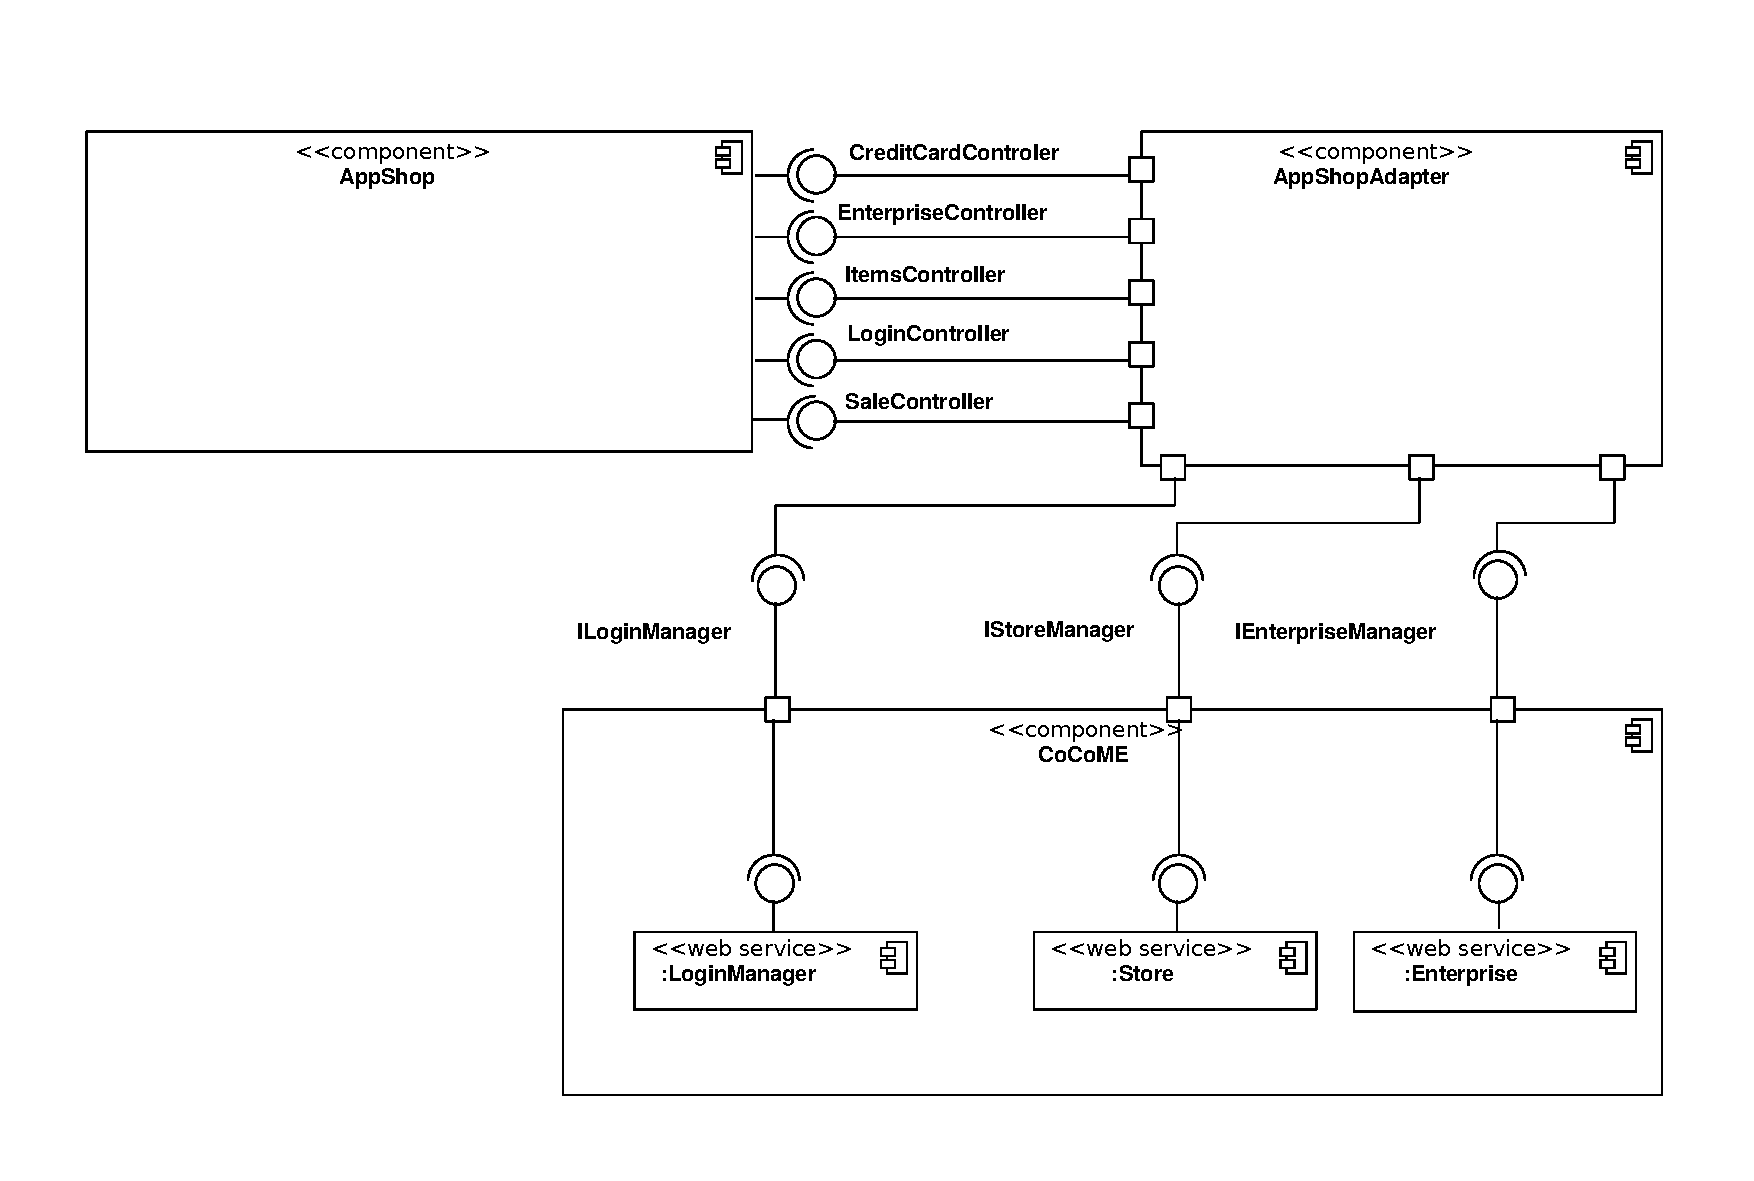
\includegraphics[width=\textwidth]{img/appComponent.pdf}
	\caption{Component Diagram of the \CoCoME Ecosystem \deleted{A}after \deleted{A}adding the Mobile App Client}
	\label{ComponentApp}
\end{figure}

The \textit{AppShopAdapter} consumes the three web services \textit{WebService::Inventory::LoginManager}, \textit{WebService::Inventory::Store}, and \textit{WebService::Inventory::Enterprise}3
Additionally, the \textit{AppShopAdatper} provides a \deleted{Rest}\added{REST} \deleted{Api}\added{Interface} which is used by the \deleted{actual }\textit{AppShop}. 
The \deleted{Rest}\added{REST Interface}\deleted{Api contains} \added{provides} endpoints to retrieve and process Credit Card, Enterprise and StockItem information. 
To implement the use cases \emph{UC14-16} the \deleted{Api }\deleted{Rest}REST Interface also provides endpoints for user management and processing sales. 
  
\begin{figure}[!h]
	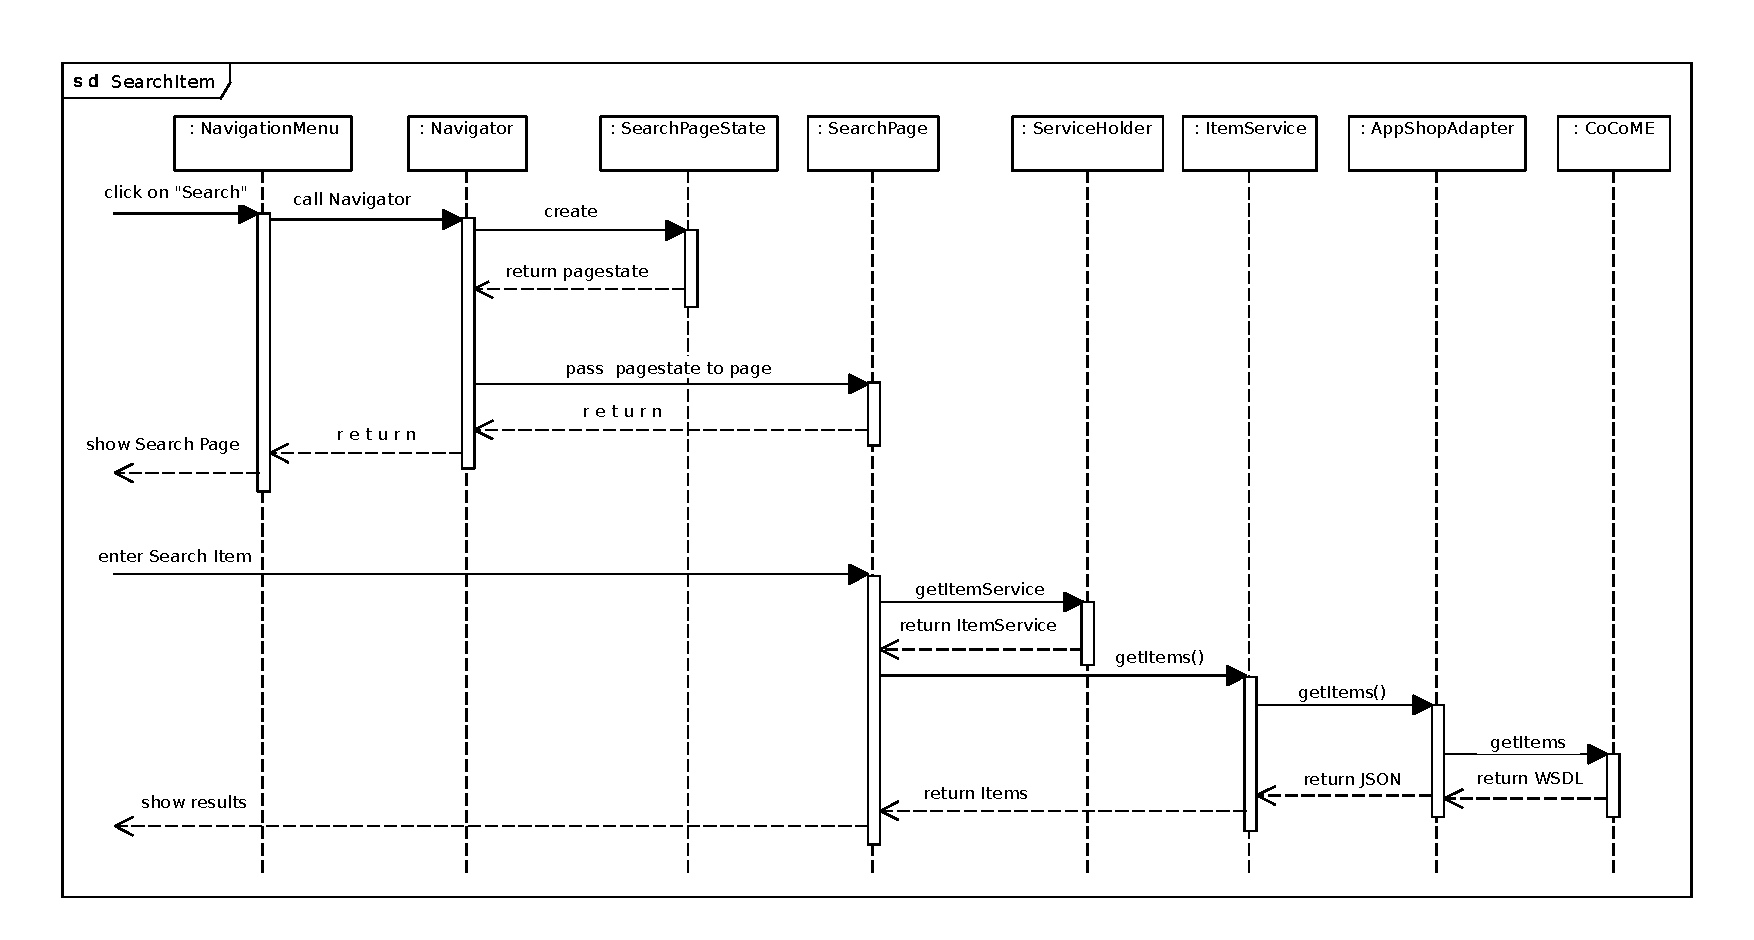
\includegraphics[width=\textwidth]{img/appSearchSequence.pdf}
	\caption{Sequence Diagram of Searching an Item in the Mobile App Client}
	\label{SequenceAppSearch}
\end{figure}

Fig.~\ref{SequenceAppSearch} shows the process of opening a page to search for an Item. 
The customer opens the \textit{WebShopClient} and triggers the "Search" function to search for an item. 
To open the page the \textit{NavigatorMenu} must call the \textit{Navigator} which creates a pagestate object and passes the object to the page. 
This HTML page is \deleted{now}then presented to the customer. 
To fill the page with information (i.e., when searching for a \textit{ProductItem}) the page uses services provided by the \textit{ServiceHolder}. 
In this case, the \textit{ItemService} calls the responsible REST-Service of \textit{AppShopAdapter} which in turn retrieves the necessary information from the WSDL services provided by \CoCoME.

Fig.~\ref{SequenceAppSale} demonstrates how the Mobile App Client processes sales. 
For the sake of clarity, the di\added{a}gram is simplified and only contains the most important calls. 
First, the customer searches for items (according to Fig.~\ref{SequenceAppSearch}). 
By clicking on the desired \deleted{I}\added{i}tem, the according \textit{ItemPage} is shown. 
\deleted{This}The \textit{ItemPage}\deleted{ page} carries information about the \deleted{I}\added{i}tem. 
Here, the customer decides whether the \deleted{I}\added{i}tem should be added to the \deleted{S}\added{s}hopping \deleted{C}\added{c}art or not. 
%Hier das TODO bearbeitet
If the customer wants to add more \textit{Items} to the shopping cart, s/he needs to repeat the last steps. This includes searching for an item, clicking on it and decided whether or not the Item should be added to the shopping cart.
%The last steps\todosk{welche genau?} are repeated until the customer decides to proceed to the checkout. 
If not logged in the customer gets forwarded to the \textit{LoginPage}. 
When successfully logged in the customer clicks the \textit{BuyNow}-Button. 
The \deleted{i}\added{s}ale process is finished as soon as the backend (\CoCoME) has processed the sale.


\begin{figure}[!h]
	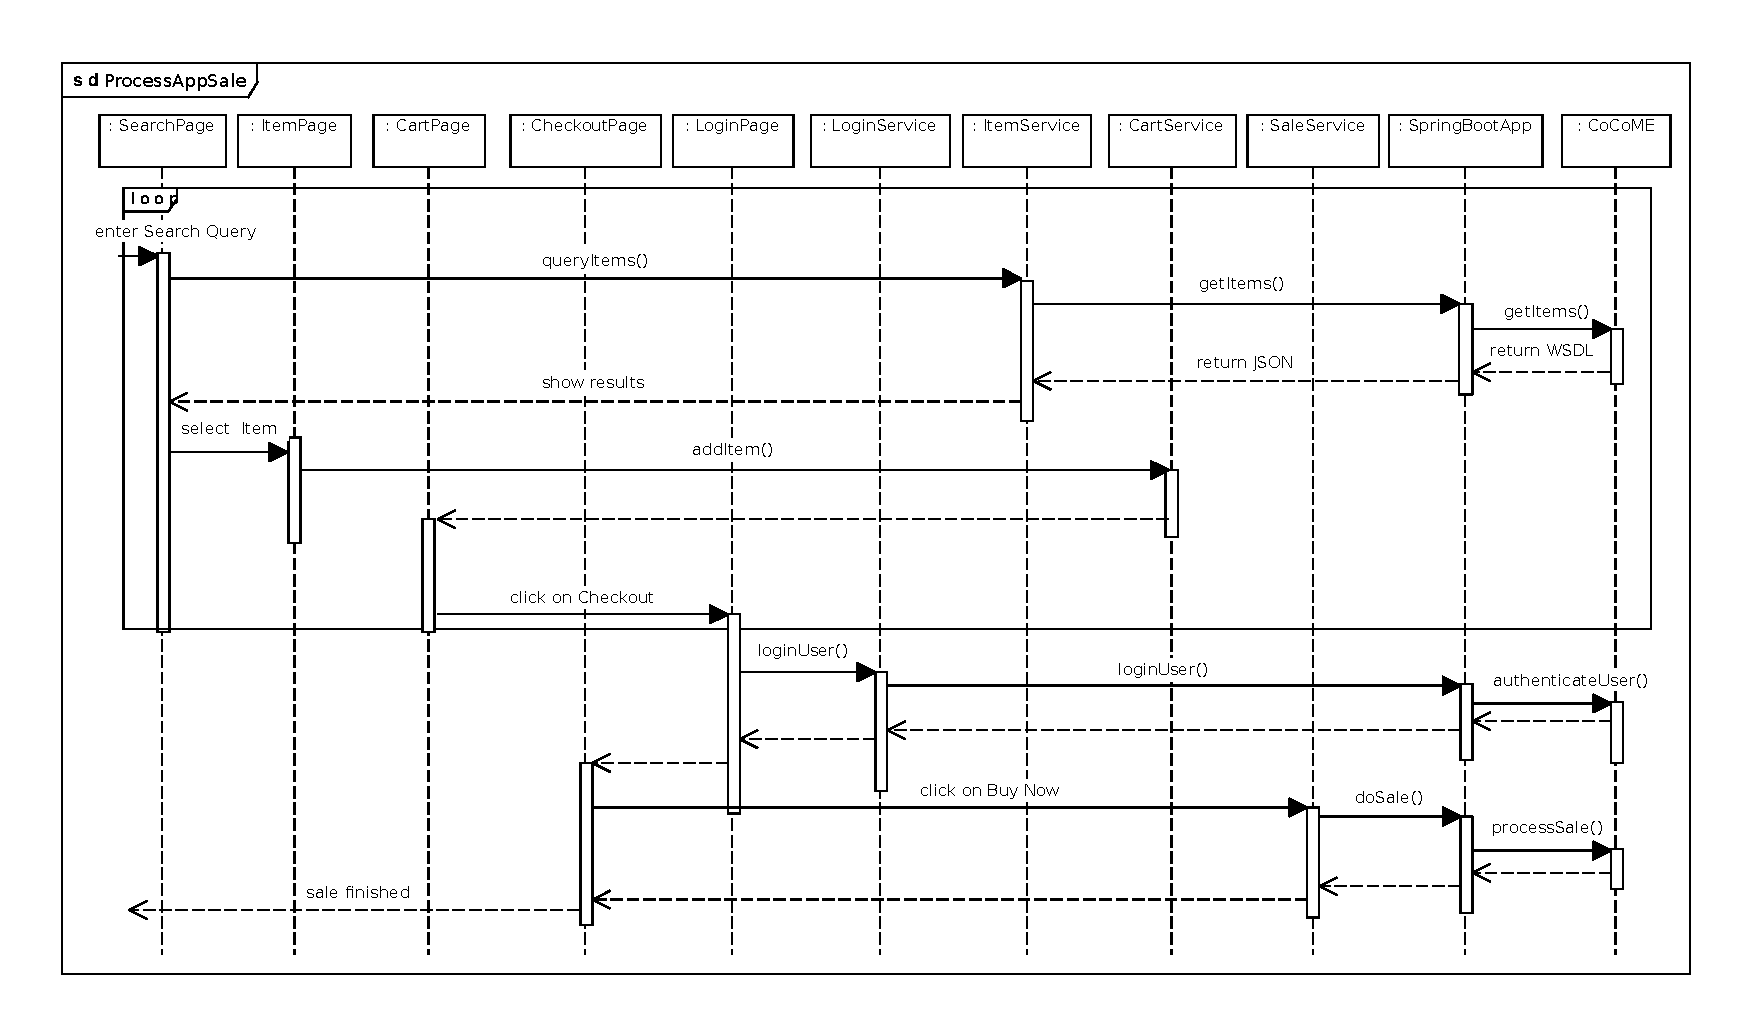
\includegraphics[width=\textwidth]{img/appProcessSale.pdf}
	\caption{Sequence Diagram of \deleted{P}\added{p}rocessing a \deleted{S}\added{s}ale}
	\label{SequenceAppSale}
\end{figure}

\newpage

\section{Using a Docker Environment} \label{Docker}

As shown in Fig.~\ref{techStack}, using a Docker Environment affects the technology stack by adding additional layers. 
\added{The \CoCoME stack consists of GlassFish, Java Virtual Machine (JVM) and Maven.}
More detailed, the given \CoCoME \deleted{S}\added{s}tack is moved into \deleted{the}\added{a} Docker \deleted{Deamon}\added{Container} which runs a Linux distribution. 
The original parts of the stack, like GlassFish and the , \deleted{Java Virtual Machine}\added{JVM} are still \deleted{a part of the stack}\added{functioning as before}.
	
	\begin{figure}[!h]
		\centering
		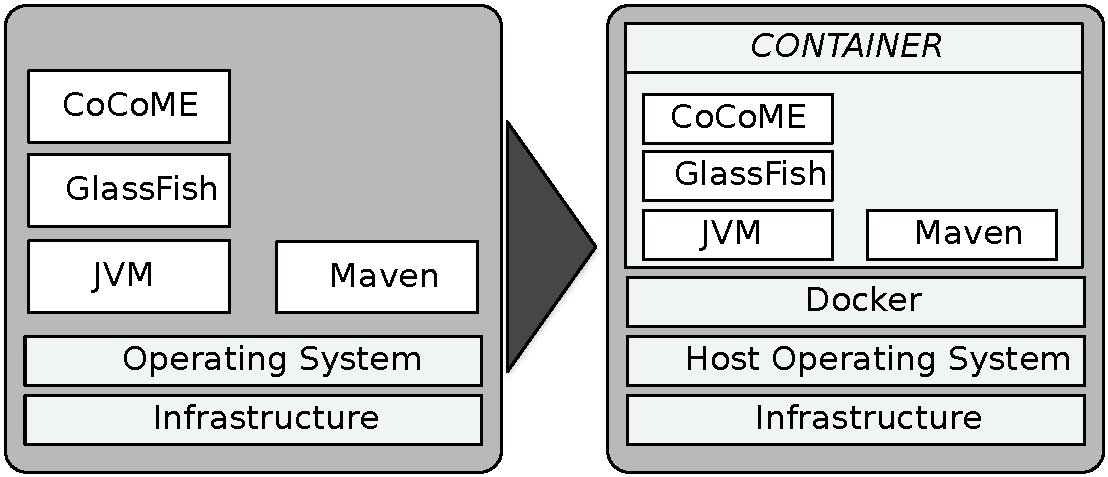
\includegraphics[width = 0.7\textwidth]{img/tech_stack_CoCoME.pdf}
		\caption{Extended technology stack \CoCoME}
		\label{techStack}
	\end{figure}
\noindent	
The Dockerfile defines an environment based on the latest version of the Linux distribution Ubuntu.
Maven, Git and Java are also installed using the standard Ubuntu package manager. %\{welche versionen von maven, git und java?}.
Git \deleted{has}serves two purposes: On the one hand it is used to download the most recent version of \added{the} \CoCoME \added{source code or a precompiled \CoCoME version}.
On the other hand, it is used to download a prefabricated version of GlassFish that is already \added{tailored to the needs of the \CoCoME application}\deleted{includes domains and other adjustments required for \CoCoME}. 
Java is required by GlassFish and \CoCoME as they need the \deleted{Java Virtual Machine}\added{JVM}. 
Maven is needed to \added{build and} deploy the latest version of \CoCoME onto the provided GlassFish servers.

During the development\added{ phase}\deleted{, it was}\added{ we} decided to implement and provide two different versions\added{ of the \CoCoME Docker Container}. 
The first version always pulls the most recent \CoCoME source code from GitHub, downloads the entire dependencies with Maven, compiles and builds the project and finally deploys \CoCoME on the GlassFish servers. 
As a consequence, creating and starting the Docker Container \added{for \CoCoME} takes about one hour.


In contrast, the second version \added{of the \CoCoME Docker Container}\deleted{only }pulls a prefabricated version of \CoCoME from GitHub. 
Therefore, pulling the source code \deleted{up }to build\deleted{ing} the \CoCoME project is skipped. 
Maven does not have to be included in the technology stack. 
Solely, deploying \CoCoME on the GlassFish server is necessary.
This reduces the deployment time to a few minutes.\deleted{ but has a disadvantage: }
\added{Nevertheless,} the prefabricated version of the GlassFish Servers and \CoCoME has to be updated manually. 
Thus, it is sometimes not the most recent version.
By providing both, a fast deploying version and a current version, the user can choose what\deleted{'s}\added{ suits best for his/her needs}\deleted{ situation}.
	

	

	
\section{Microservices Technology} \label{MS}
In this section we provide a brief design documentation of the use cases that are defined in the hybrid cloud-based variant of \CoCoME~\cite{herold2008}(p.4-10).
The following subsections are divided into the \deleted{M}\added{m}icroservices and the corresponding use cases. 
Sec.\ref{archiOverviewMicro} describes the general architectural overview of the \deleted{M}\added{m}icroservice variant of \CoCoME.
	



	\FloatBarrier
		\subsection{Orders}
		This section describes the design of the use cases implemented in the \textit{Orders} \deleted{M}\added{m}icroservice\added{.}
		\added{T}\deleted{t}hat service provides main parts of the functionality for UC 3 and UC 4.

		\subsubsection*{Behavio\deleted{u}ral View on UC 3 - Order Products} 
		For \added{a} better understanding, UC 3 is divided in two steps. The first part is described in Fig.~\ref{MS_UC3_1}: A user chooses the product items \added{and amount }to order.\deleted{ and the corresponding amount.} Each \textit{ProductOrder} is stored in the \textit{ProductOrderRepository} as a \textit{OrderEntry}. In the second part (Fig.~\ref{MS_UC3_2}), the \textit{OrderEntries} are wrapped in a single \textit{ProductOrder} element\deleted{ that a}\added{. A}dditionally\added{, the \textit{ProductOrder} element} contains information about the store and the date of the order. When the user presses the button \textit{Order}, the \textit{OrderManagement} iterates over the collection of \textit{OrderEntries} and sets a reference to the actual \textit{ProductOrder}.
	

		
			\begin{figure}[!h]
				\centering
				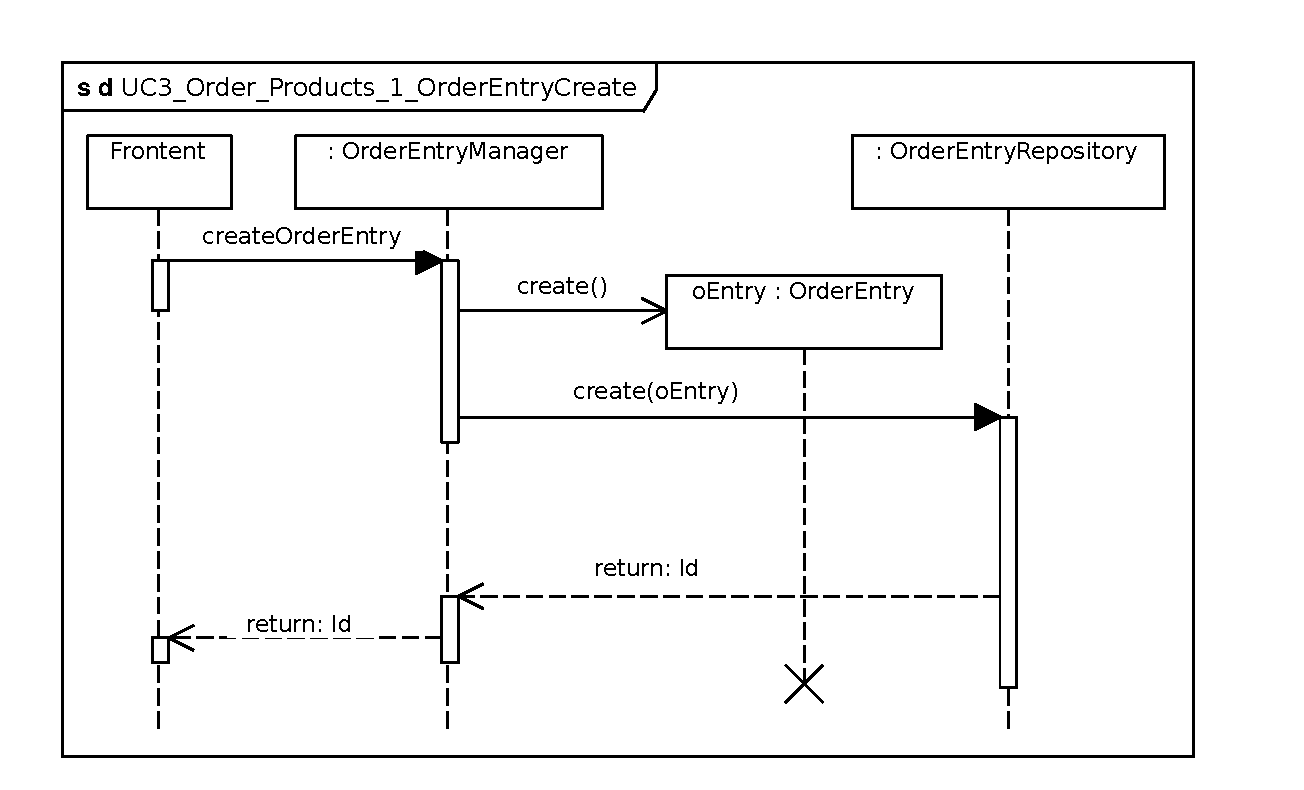
\includegraphics[width = 0.7\textwidth]{img/UC3_Order_Products_1_OrderEntryCreate.pdf}
				\caption{UC 3: \textit{Order Products} (part 1)}
				\label{MS_UC3_1}
			\end{figure}
			
			\begin{figure}[!h]
				\centering
				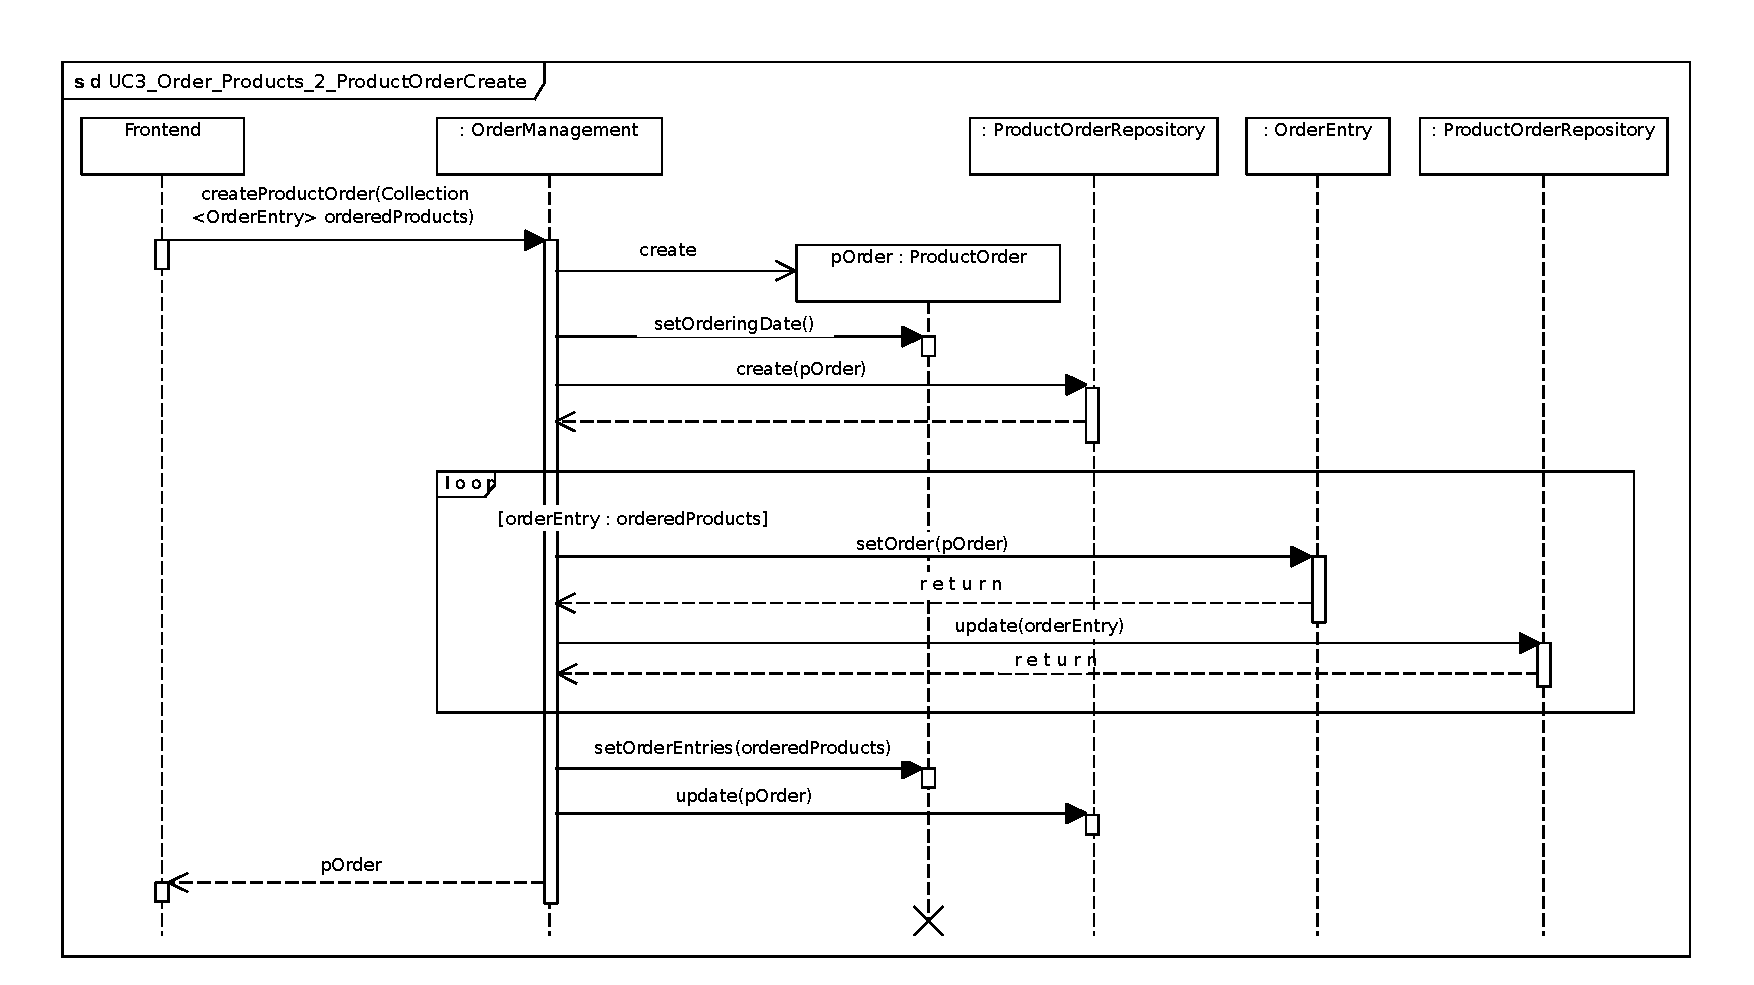
\includegraphics[width = 1\textwidth]{img/UC3_Order_Products_2_ProductOrderCreate.pdf}
				\caption{UC 3: \textit{Order Products} (part 2)}
				\label{MS_UC3_2}
			\end{figure}
		
		\subsubsection*{Behavio\deleted{u}ral View on UC 4 - Receive Ordered Products}
		Fig.~\ref{MS_UC4} shows\deleted{, that first} the \textit{ProductOrder} element\added{.}
		\added{It}\deleted{, which handles the order with the passed \deleted{id}\added{\textit{Id}},} is refreshed and the delivery date is set to the passed date.
		\added{The \textit{ProductOrder} element handles the order regarding the containing \textit{Id}.}
		After this, it performs for each \deleted{OrderEntry}\added{\textit{OrderEntry}} a rest call to the store microservice. With that \added{REST}\deleted{rest} call the \added{number of }\deleted{StockItem}\added{\textit{StockItems}}\deleted{, which is representing the \deleted{corresponding }product in the store,} is increased \added{by }the amount of delivered products.
		\added{\textit{StockItems} representing a concrete product within the system}.
			
			\begin{figure}[!h]
				\centering
				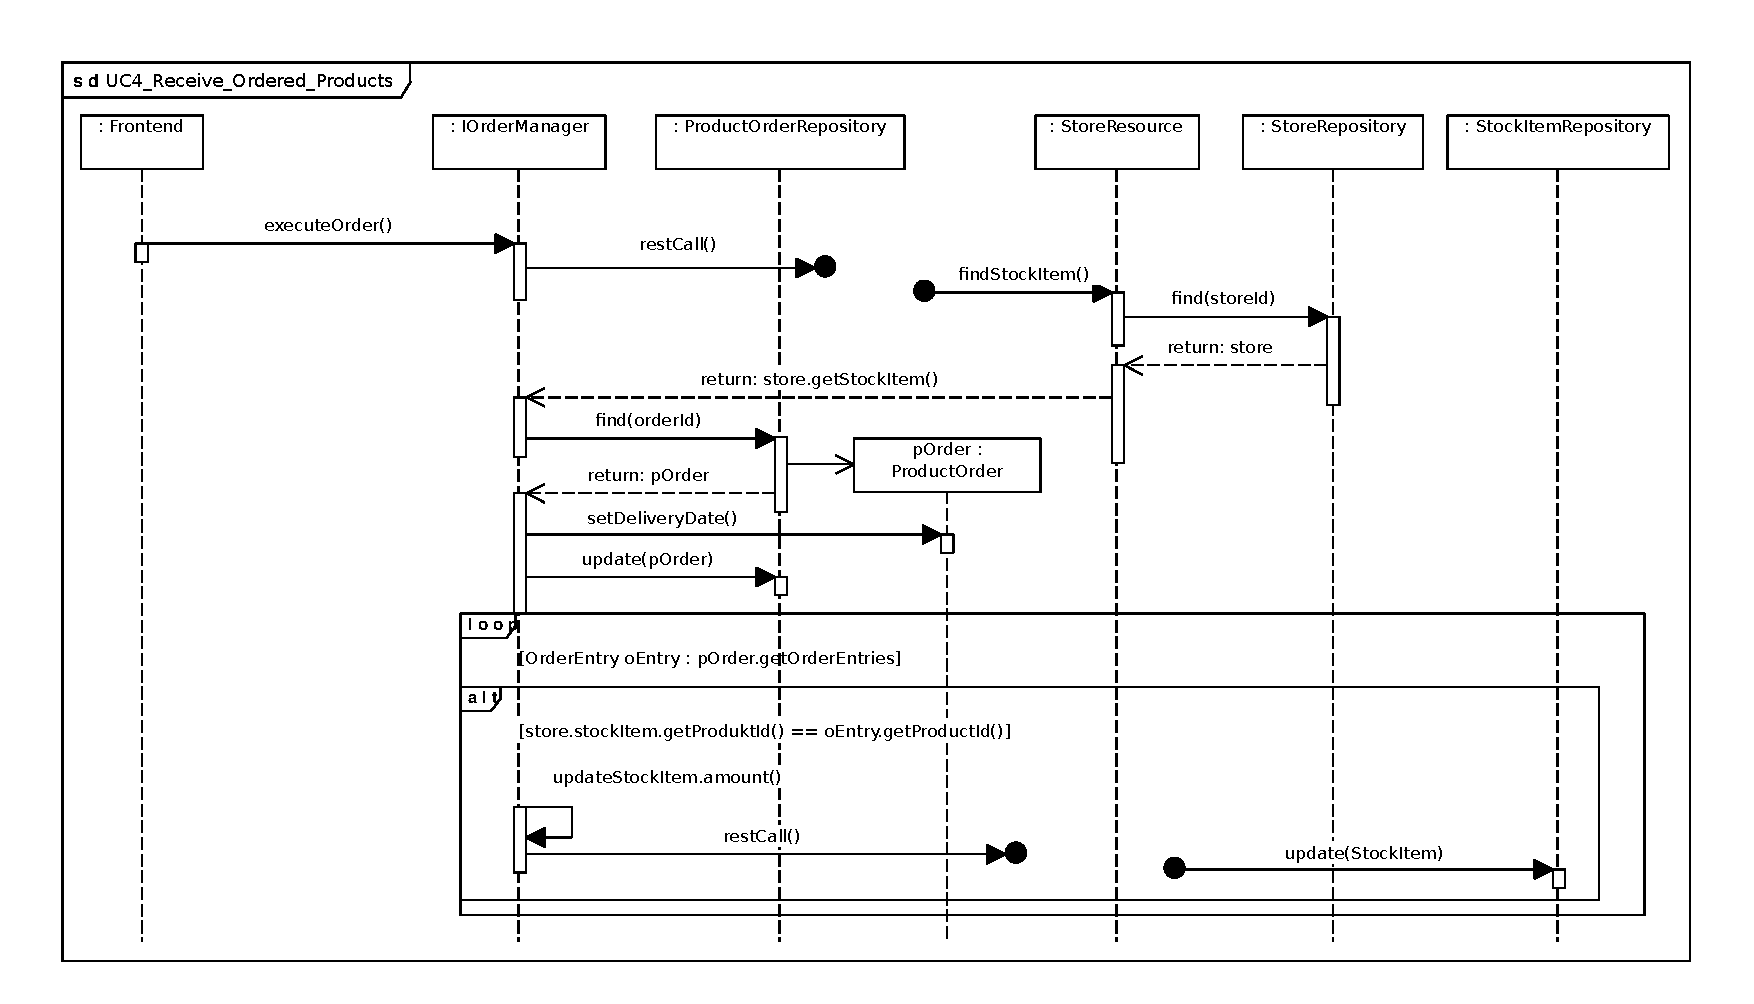
\includegraphics[width = 1\textwidth]{img/UC4_Receive_Ordered_Products.pdf}
				\caption{UC 4: \textit{Receiver Ordered Products} }
				\label{MS_UC4}
			\end{figure}
			
		\FloatBarrier
			
		\subsection{Stores}
			This section describes the design of the use cases implemented in the \textit{Store} \deleted{M}\added{m}icroservice that provides main parts of the functionality for UC 1, UC 2, UC 7 and UC 8.

		\subsubsection*{Behavio\deleted{u}ral View on UC 1 - Process Sale} 
		Again, UC 1 is divided in two parts (Fig.~\ref{MS_UC1_1} and Fig.~\ref{MS_UC1_2}).
		The first part describes how a user can add products to the sale process. When the \textit{startSale} action is executed, the sale mode is activated and the \textit{CashDesk} is resetted from a previous, probably cancel\deleted{l}ed sale processes. To add products to the sale process, the user can either enter the barcode \deleted{digit by digit}\added{manually} using the keyboard or scan the barcode using a \textit{Scanner}. Further, the user can choose how many products s/he wants to purchase. This process is depicted in the inner loop. 
		
		Several checks are executed when successfully entering the barcode: \added{The scanned item must exist in the system. }
		If an item with the same barcode was already added to the sale, then the\deleted{ actual} total \textit{inventoryAmount} is increased by the second purchase amount. 
		If \deleted{not,}\added{no item with the same barcode is present, }the scanned item is added to the sale.
		\deleted{provided that an item with this barcode exists.}In both cases, the availability \added{and the amount }of the item\deleted{ amount} in the stock is checked and reduced. 
		If one of the conditions is violated, the attempt of adding a product with the provided barcode and amount is \deleted{quit}\added{aborted}. 
		Subsequently, the display is updated and the product information is added to the printer output.
		
		The second part of this use case, shown in Fig.\added{~}\ref{MS_UC1_2}, handles the end of the sale process. 
		\added{The \textit{finishSale} routine is called when the \textit{FinishSale} button is pressed.}\deleted{By calling the \textit{finishSale} routine (when pressing the button \textit{FinishSale}), the display is updated.}
		\added{Thus, the display gets updated.}
		Now, the user needs to choose between paying by card or cash and the \textit{CashDesk} is set to the corresponding paying mode. 
		In case the user wants to pay by credit card, s/he needs to enter the credit card details. 
		In the other case, the cash amount is entered. 
		In both cases, the information is checked \deleted{to}\added{for} accuracy.
		After successfully ending the payment, the printer and display are updated and the \textit{CashDesk} ends the sale process.

		\subsubsection*{Behavioral View on UC 2 - Manage Express Checkout}
		Changing the express mode is triggered on two occasions (\textit{externalCall}). 
		First, when finishing a sale and if, as descibed in \cite{herold2008}, some customizable terms regarding previous sales are fulfilled, the \textit{CashDesk} switches into express mode automatically.\\ These conditions can for example be an average of 4 goods per selling process during the past ten selling processes.\\
		Second, the Cashier \added{switches manually back to normal mode.}\deleted{is able to switch back to normal mode.}
		In both cases, the \textit{updateExpressLight} routine checks the current \textit{ExpressLight} state and performs an update in accordance with the kind of call.
		
		\subsubsection*{Behavio\deleted{u}ral View on UC 7 - Change Price}
		The \textit{StoreManager} is able to change a price for \textit{StockItems} that are available in his/her store. 
		As depicted in Fig.~\ref{MS_UC7}, the \textit{StoreAdminManager} selects the right \textit{Store}, based on the \textit{StoreManager} that is logged in. 
		To find the correct \textit{StockItem}, the available items are filtered by a given product id. 
		When the correct \textit{StockItem} is found, the sale price can be simply updated by entering the new price. 
		Finally, the \textit{StockItem} in the database is updated.
		
		\subsubsection*{Behavio\deleted{u}ral View on UC 8 - Product Exchange}
		In case a Store is going to run out of a certain \textit{StockItem}, products from a different \textit{Store} within the same Enterprise can be exchanged. 
		The process is triggered at the end of a sale. 
		It is shown in  Fig.~\ref{MS_UC8}. 
		The \deleted{M}\added{m}icroservice \textit{Store} checks if the stock amount of the sold items have passed the minimal stock amount. 
		If \deleted{not, nothing happens. 
		Otherwise,}\added{the minimal stock amount is passed,} the \deleted{S}\added{s}ystem calls the \textit{shiftItem} routine. 
		First, all \textit{Stores} within the same \textit{Enterprise} of the \textit{Store} that is running out of stock are collected.
		For each \textit{Store}, the system checks if the desired \textit{StockItem} is available. 
		The \textit{findOptimum} routine decides \deleted{(using heuristics) }whether the transportation is meaningful. 
		\added{Therefore, heuristics are used.}
		After a successful query, the \textit{StockItem} is shipped from one Store to another, decreasing the amount at the first \textit{Store} and increasing it at the second.

		
			\begin{figure}[!h]
				\centering
				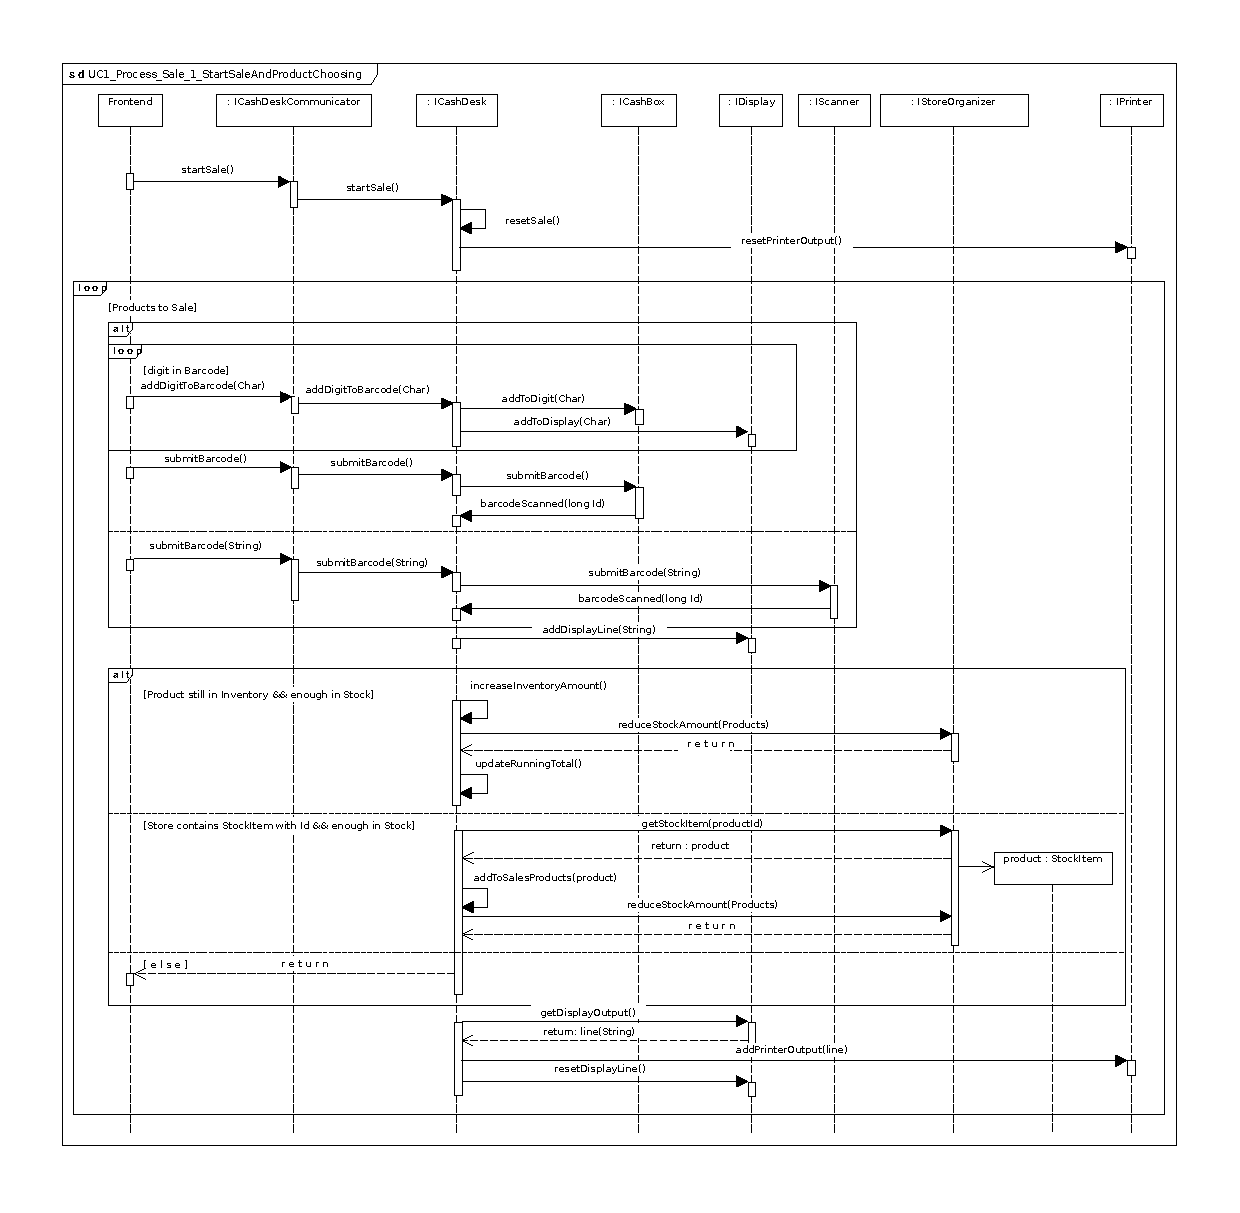
\includegraphics[width = 1\textwidth]{img/UC1_Process_Sale_1_StartSaleAndProductChoosing.pdf}
				\caption{UC 1: \textit{Process Sale} (part 1)}
				\label{MS_UC1_1}
			\end{figure}
			
			\begin{figure}[!h]
				\centering
				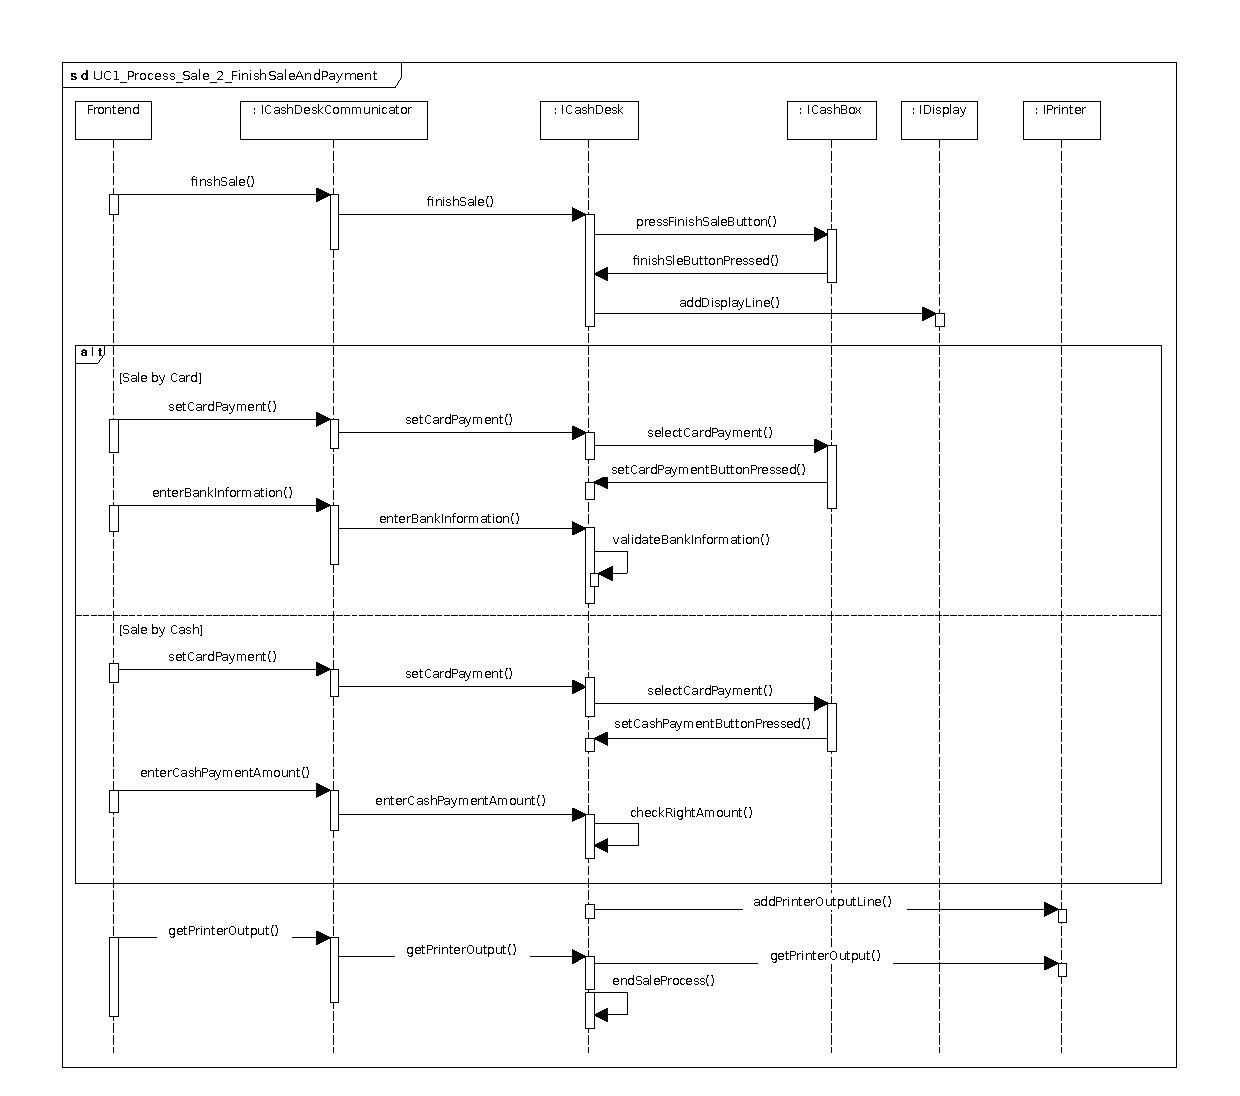
\includegraphics[width = 1\textwidth]{img/UC1_Process_Sale_2_FinishSaleAndPayment.pdf}
				\caption{UC 1: \textit{Process Sale} (part 2)}
				\label{MS_UC1_2}
			\end{figure}
			
			\begin{figure}[!h]
				\centering
				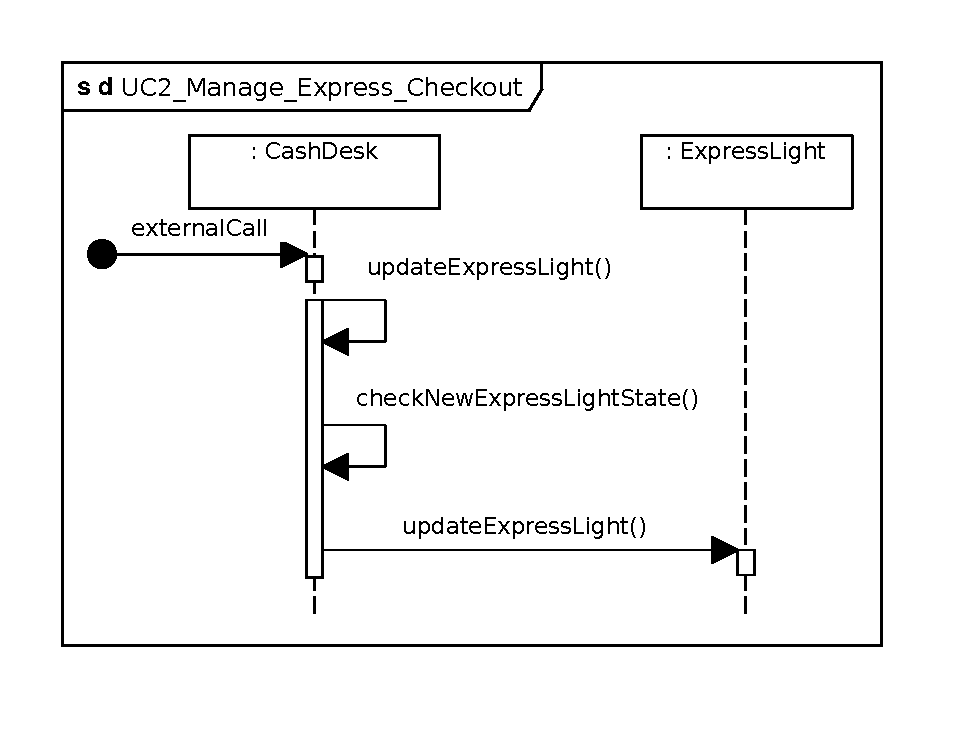
\includegraphics[width = 0.5\textwidth]{img/UC2_Manage_Express_Checkout.pdf}
				\caption{UC 2: \textit{Manage Express Mode}}
				\label{MS_UC2}
			\end{figure}
			
			\begin{figure}[!h]
				\centering
				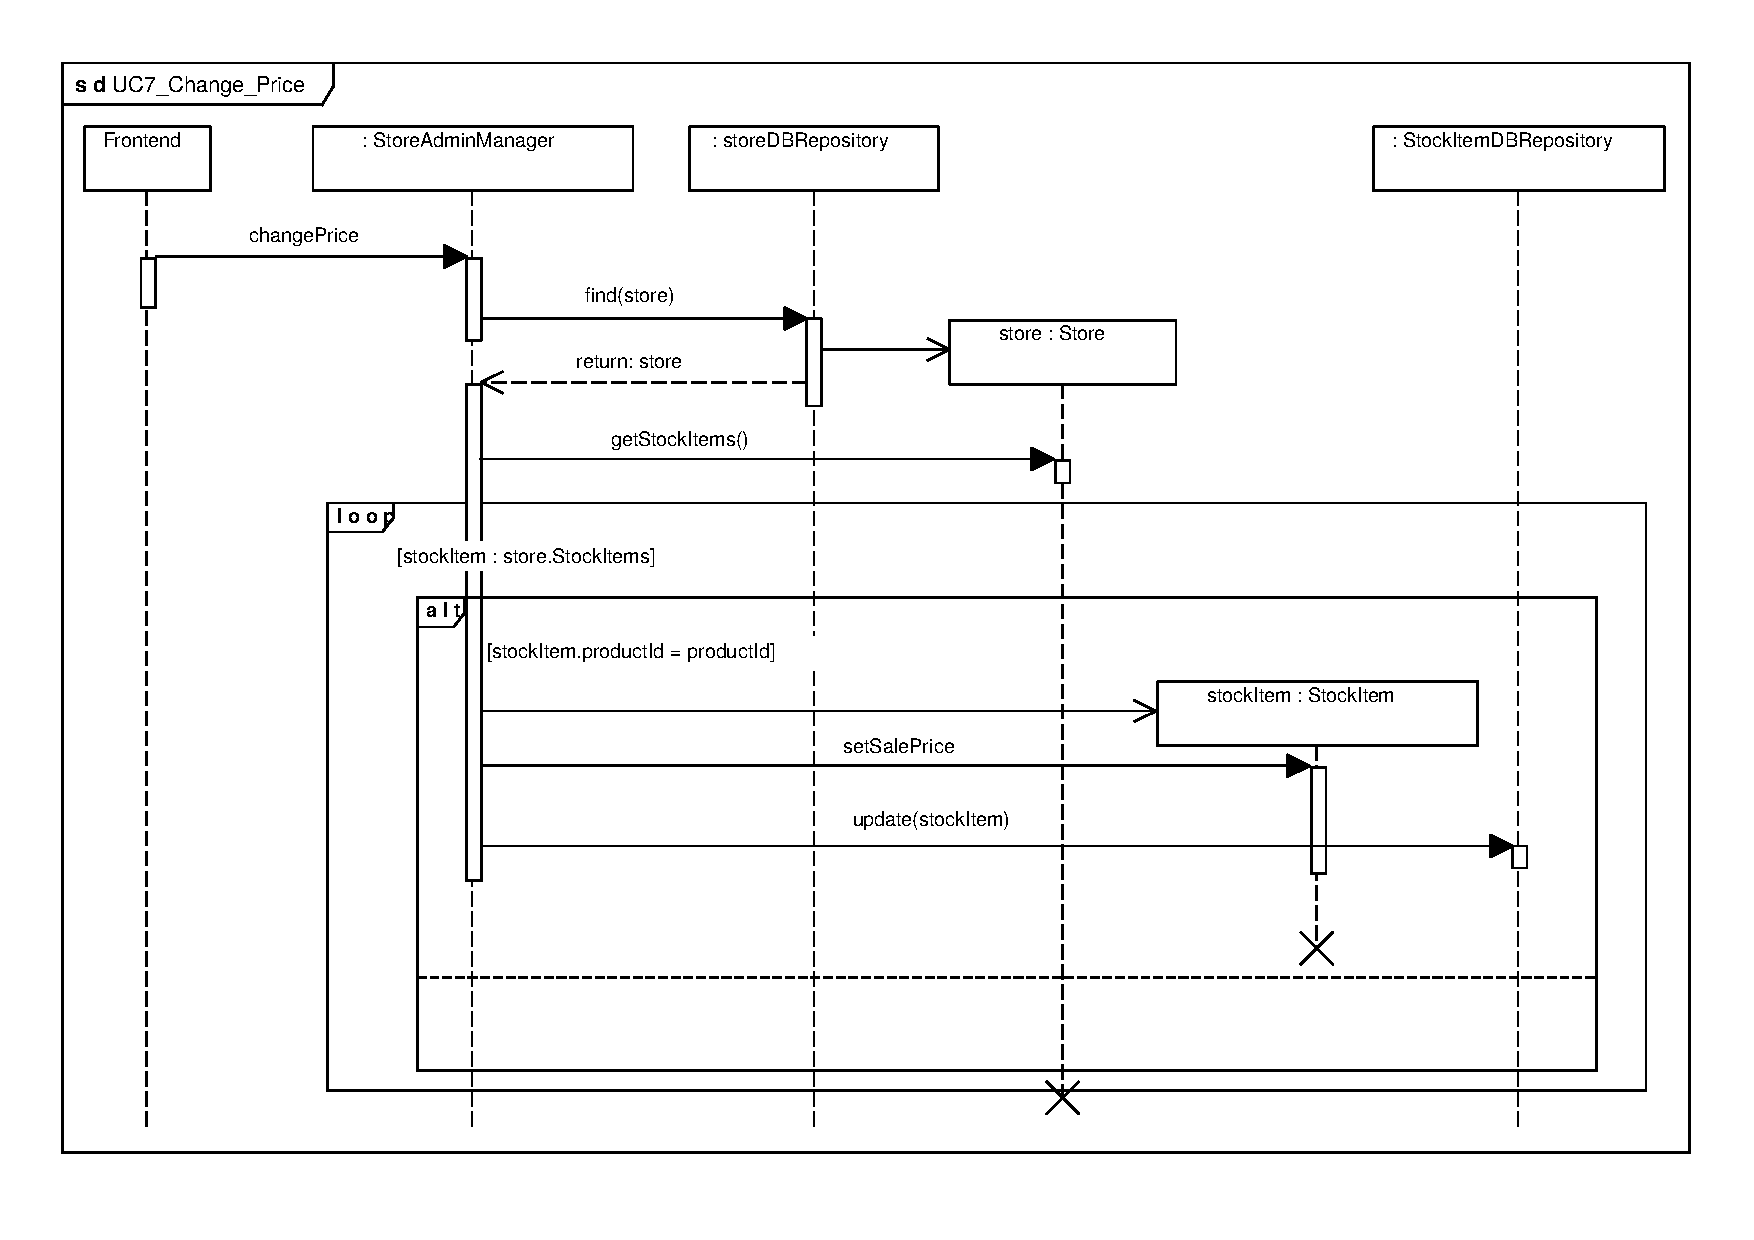
\includegraphics[width = 0.9\textwidth]{img/UC7_Change_Price.pdf}
				\caption{UC 7: \textit{Change Price}}
				\label{MS_UC7}
			\end{figure}
			
			\begin{figure}[!h]
				\centering
				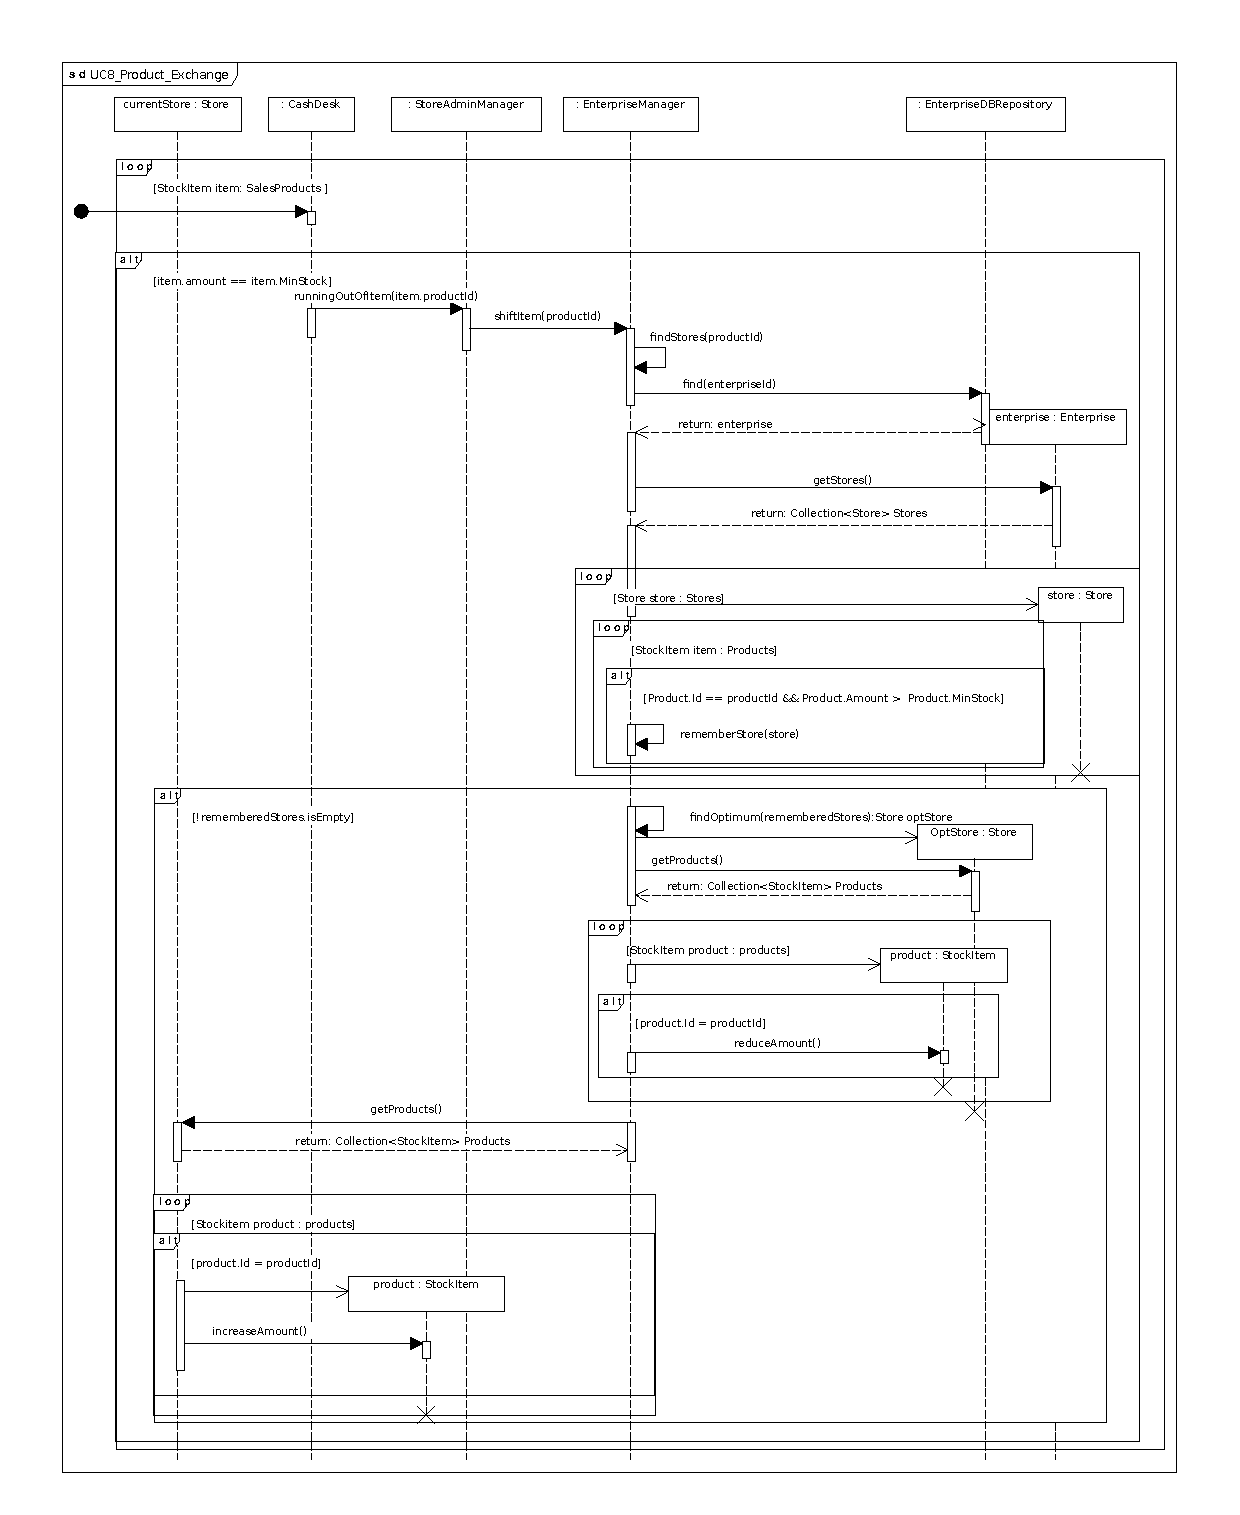
\includegraphics[width = .9\textwidth]{img/UC8_Product_Exchange.pdf}
				\caption{UC 8: \textit{Product Exchange}}
				\label{MS_UC8}
			\end{figure}
		\FloatBarrier	
		
		\subsection{Reports}
		This section describes the design of the \textit{Reports} \deleted{M}\added{m}icroservice, which provides the functionality of the UC 5 and 6.
		
		\textbf{Behavio\deleted{u}ral View on UC 5 and UC 6 - Show Stock Report and Show Delivery Report} 
		The \textit{StoreManager} can request a full \textit{StockReport} that includes all available stock items in the store. 
		This process is described \deleted{as}\added{in the use case} UC 5 in~\ref{MS_UC5}. 
		The \textit{StoreManager} enters the store identifier and the \textit{StoreCommunicator} within the \textit{Reports} \deleted{M}\added{m}icroservice requests the desired information via a \deleted{rest}\added{REST} call.
		
		Besides, the \textit{Reports} \deleted{M}\added{m}icroservice provides the \deleted{opportunity}\added{functionality} to calculate the mean time\deleted{s} a delivery \added{takes} from each supplier to a considered enterprise\deleted{ takes} (UC 6). 
		The process is described in Fig.~\ref{MS_UC6}. 
		The \textit{EnterpriseManager} enters the order \deleted{id}\added{\textit{Id}} and the \textit{OrderCommunicator} requests the information as a delivery report via \deleted{rest}\added{REST} call. 
		The report is displayed to the \textit{EnterpriseManager}.
		
	
			
			\begin{figure}[!h]
				\centering
				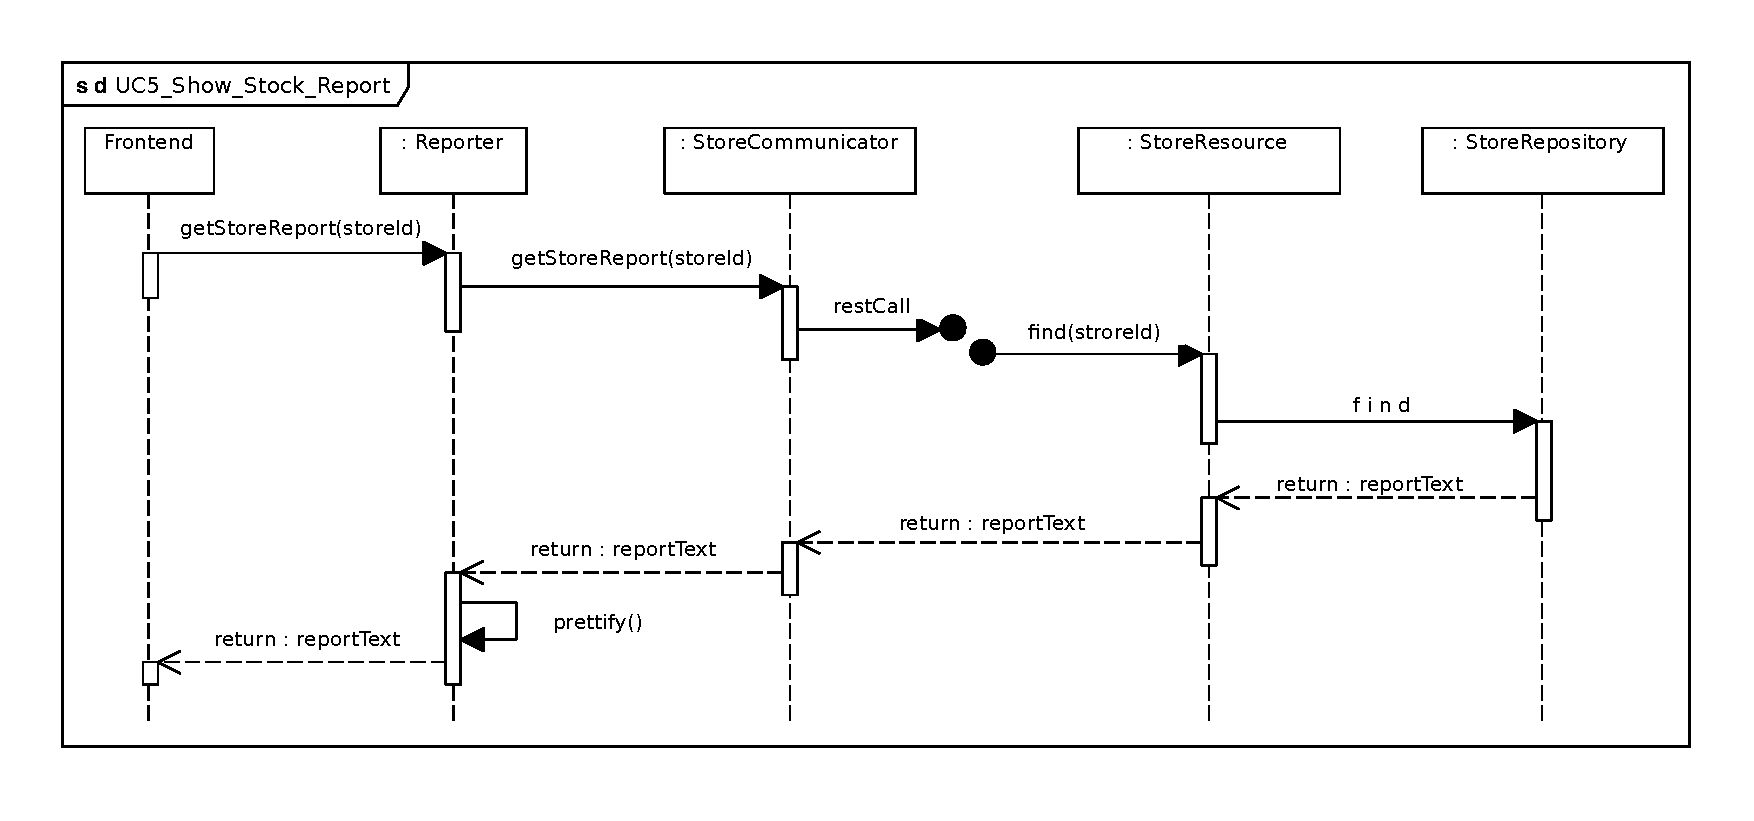
\includegraphics[width = 1\textwidth]{img/UC5_Show_Stock_Report.pdf}
				\caption{UC 5: \textit{Show Stock Report}}
				\label{MS_UC5}
			\end{figure}
			
			\begin{figure}[!h]
				\centering
				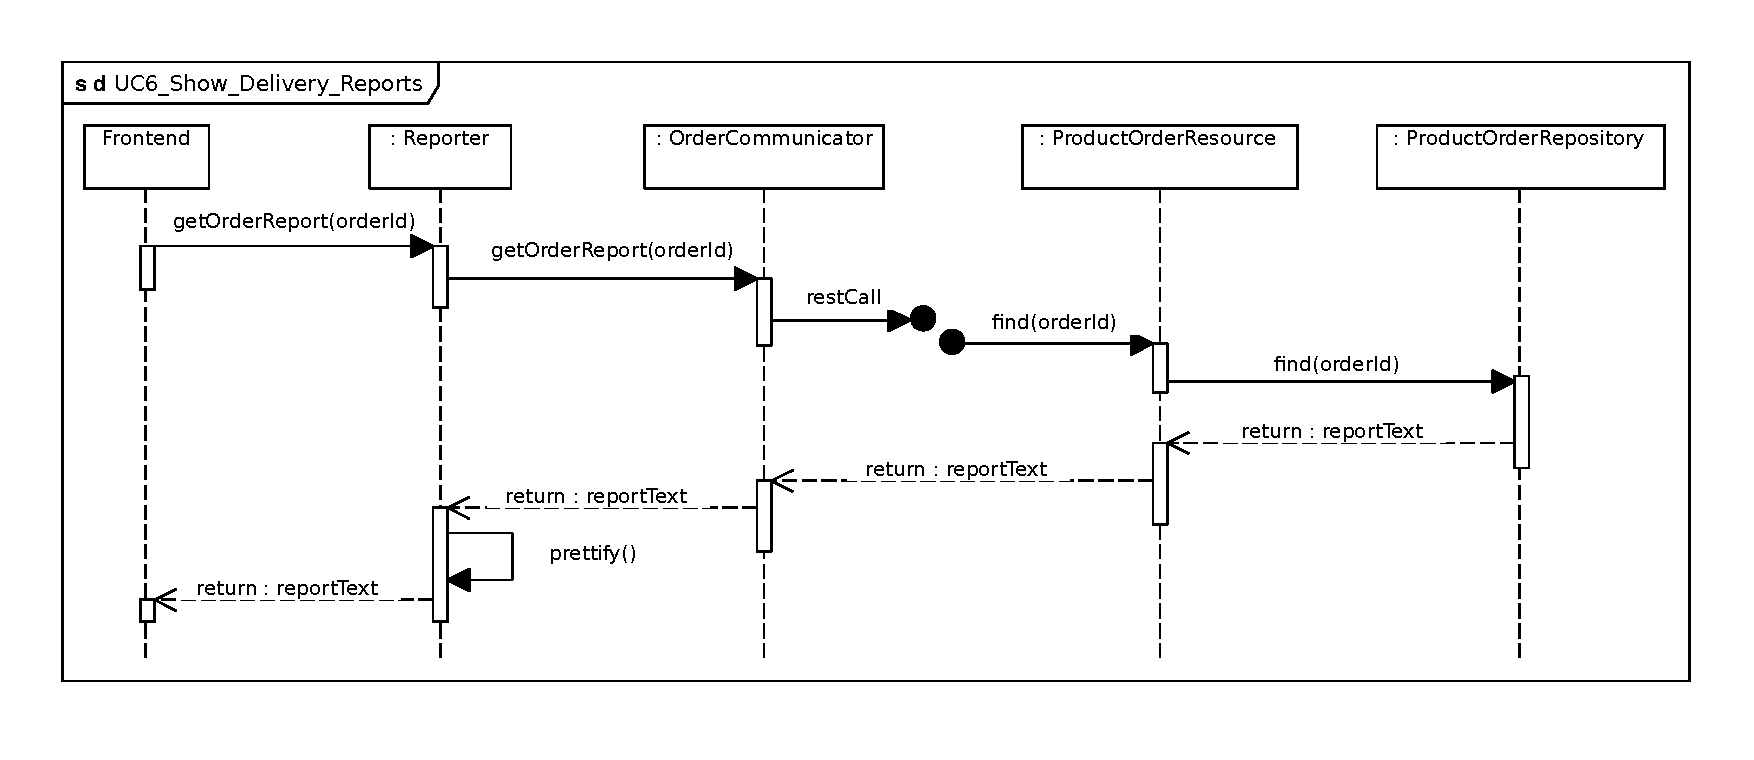
\includegraphics[width = 1\textwidth]{img/UC6_Show_Delivery_Reports.pdf}
				\caption{UC 6: \textit{Show Delivery Report}}
				\label{MS_UC6}
			\end{figure}
			
	\FloatBarrier
	\subsection{Architectural overview}	\label{archiOverviewMicro}	
	This section describes the architectural design of the \deleted{M}\added{m}icroservices. 
	\CoCoME is divided into four different \deleted{M}\added{m}icroservices: \textit{Orders}, \textit{Reports}, \textit{Stores} and \textit{Products} (Fig.~\ref{MS_ARch}). 
	Each \deleted{M}\added{m}icroservice provides its own graphical user interface\added{.}
	\added{The graphical user interface} \deleted{that }can be loaded dynamically. 
	Further, each service provides its core functionality that sometimes requires a connection to other \deleted{M}\added{m}icroservices via REST. 
	Each service apart from \textit{Reports}, has its own Database.

	The \textit{Store} service provides functionality for Store- and Enterprise Managers. 
	They can create stores, change sale prices for goods or order products. 
	For the last two functionalities, the \textit{Order} and \textit{Products} \deleted{S}\added{s}ervice is needed. 
	Further, the \textit{Store} service handles the sale process. 
	


	
	
	\begin{sidewaysfigure}[ht]
	   	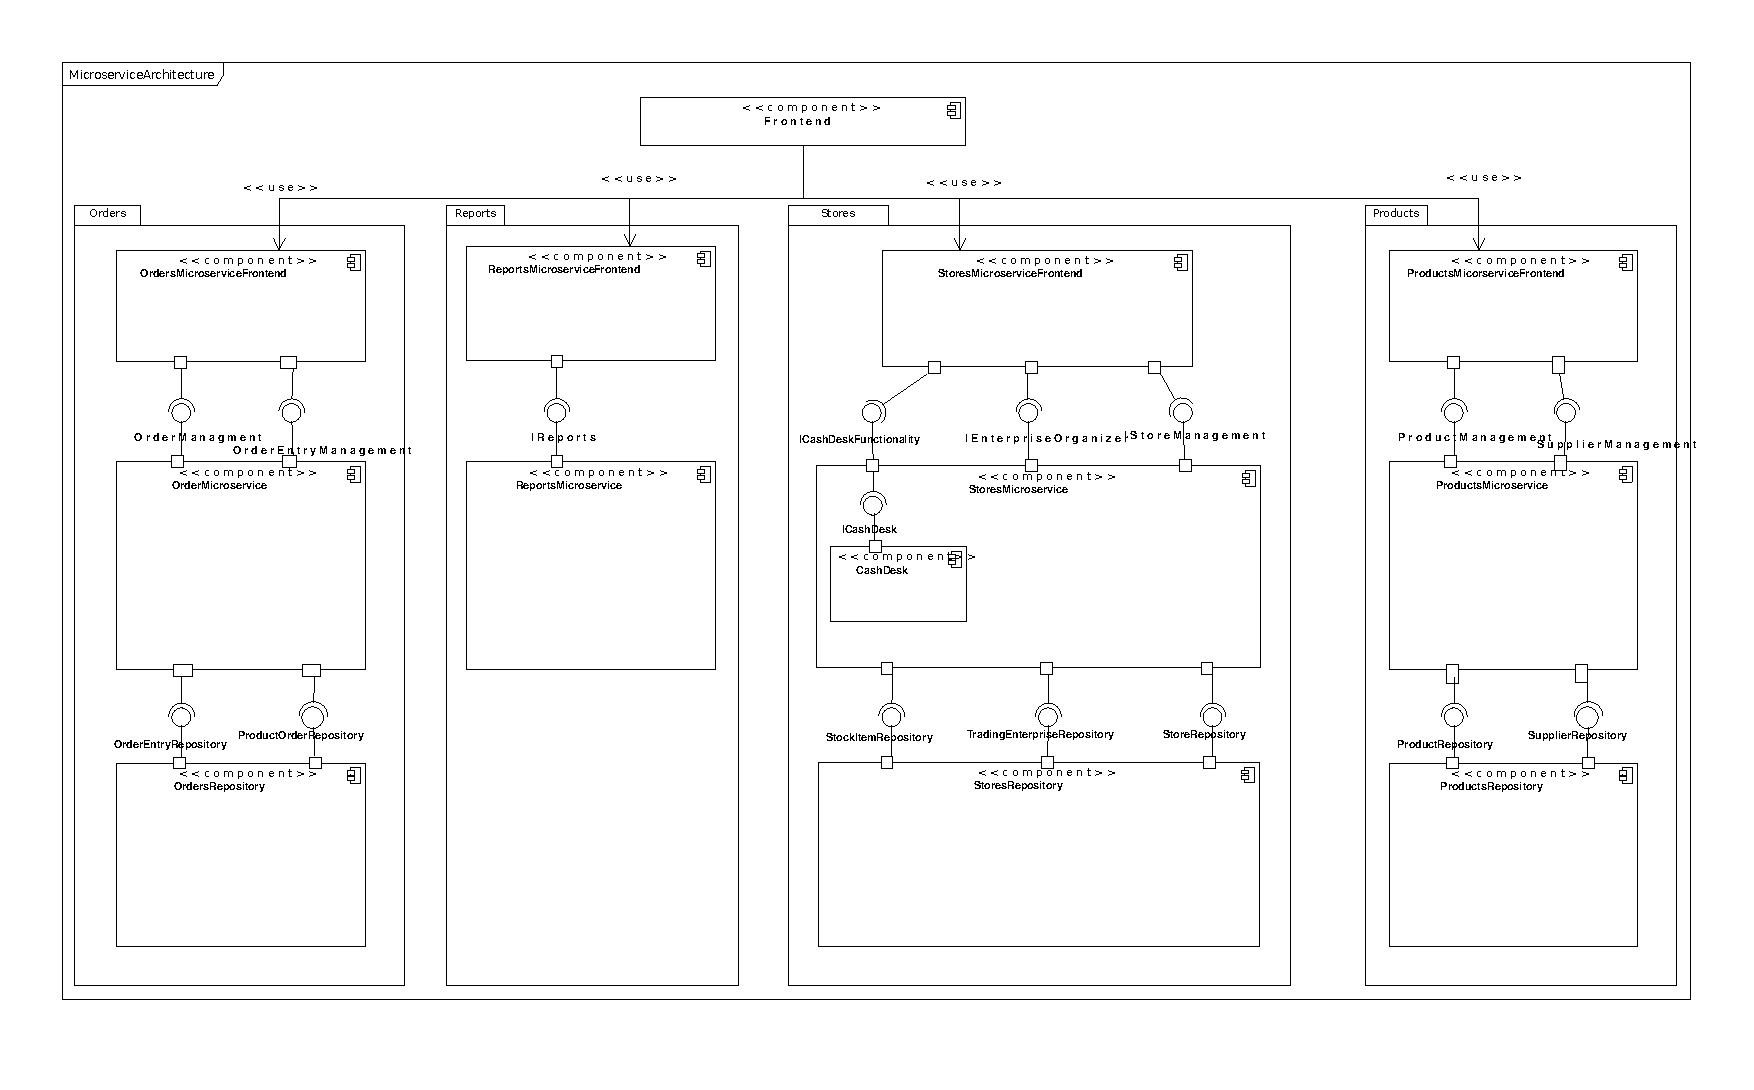
\includegraphics[width=\textwidth]{img/MicroserviceArchitecture.pdf}
	   	\caption{Microservice architecture}
	   	\label{MS_ARch}
	\end{sidewaysfigure}
